\documentclass[sigconf,10pt,anonymous]{acmart}

%% Rights management information.  This information is sent to you
%% when you complete the rights form.  These commands have SAMPLE
%% values in them; it is your responsibility as an author to replace
%% the commands and values with those provided to you when you
%% complete the rights form.
%\setcopyright{acmcopyright}
%\copyrightyear{2018}
%\acmYear{2018}
%\acmDOI{XXXXXXX.XXXXXXX}

%% These commands are for a PROCEEDINGS abstract or paper.
\acmConference[MobiCom '23]{The 29th Annual International Conference on
Mobile Computing and Networking}{October 02--06,
  2023}{Madrid, Spain}
%%
%%  Uncomment \acmBooktitle if the title of the proceedings is different
%%  from ``Proceedings of ...''!
%%
%%\acmBooktitle{Woodstock '18: ACM Symposium on Neural Gaze Detection,
%%  June 03--05, 2018, Woodstock, NY}
%\acmPrice{15.00}
%\acmISBN{978-1-4503-XXXX-X/18/06}


% Uncomment to enable anonymous submission
%\newcommand*{\ANON}{}%
% Uncomment to make the paper "submission-ready"
\newcommand*{\SUBMISSION}{}%

%  Hide URLs for anonymous submission
\ifdefined\ANON
\newcommand{\repo}{\url{https://www.dropbox.com/sh/v8ct0un8x7loi3m/AAB6op3fOWCp9qKEYlFI_Upba?dl=0}}
\newcommand{\repotamarin}{\textbf{redacted}}
\newcommand{\repoprl}{\textbf{redacted}}
\newcommand{\reposimulation}{\textbf{redacted}}
\else
\newcommand{\repo}{\url{https://github.com/EricssonResearch/v2x-self-revocation}}
\newcommand{\repotamarin}{\url{https://github.com/EricssonResearch/v2x-self-revocation/tree/main/proofs}}
\newcommand{\repoprl}{\url{https://github.com/EricssonResearch/v2x-self-revocation/tree/main/prl}}
\newcommand{\reposimulation}{\url{https://github.com/EricssonResearch/v2x-self-revocation/tree/main/simulation}}
\fi


\ifdefined\SUBMISSION
\usepackage[disable]{todonotes}
\else
\usepackage[textsize=footnotesize]{todonotes}
\presetkeys{todonotes}{fancyline}{}
\setlength{\marginparwidth}{1.3cm}
\setlength{\marginparsep}{3pt}
\fi

\newcommand{\christoph}[1]{\todo[color=orange!20]{\textbf{Christoph:} #1}}
\newcommand{\eddy}[1]{\todo[color=yellow]{\textbf{Eddy:} #1}}
\newcommand{\fritz}[1]{\todo[color=blue!20]{\textbf{Fritz:} #1}}
\newcommand{\gianluca}[1]{\todo[color=red!20]{\textbf{Gianluca:} #1}}
\newcommand{\jt}[1]{\todo{\textbf{JT:} #1}}
\newcommand{\karl}[1]{\todo[color=gray!20]{\textbf{Karl:} #1}}

\usepackage{acronym}
\usepackage{enumerate}
\usepackage{subcaption}
\usepackage{pgfplots}
\pgfplotsset{
    width=5cm, 
    legend style={
        font=\footnotesize,
        %rounded corners=2pt
    },
    compat=newest
}
\usepackage[utf8]{inputenc}
\DeclareUnicodeCharacter{2212}{−}
\usepgfplotslibrary{groupplots,dateplot}
\usetikzlibrary{patterns,shapes.arrows}
% timeline diagram
\usetikzlibrary{decorations.pathreplacing,calligraphy}

\usepackage[cmex10]{amsmath}
\usepackage{url}
\usepackage{tabularx}
\usepackage{fontawesome}

%\titleformat{\paragraph}[runin]
%{\bfseries}{\theparagraph}{1em}{}

\newtheorem{req}{Requirement}
\newtheorem{defn}{Definition}
\newtheorem{prop}{Property}

\usepackage[capitalize]{cleveref}
\crefname{figure}{Fig.\@}{Figs.\@}
\Crefname{figure}{Fig.\@}{Figs.\@}
\crefname{table}{Tab.\@}{Tabs.\@}
\Crefname{table}{Tab.\@}{Tabs.\@}
\crefname{section}{Sect.\@}{Sects.\@}
\Crefname{section}{Sect.\@}{Sects.\@}
\crefname{req}{Req.\@}{Reqs.\@}
\Crefname{req}{Req.\@}{Reqs.\@}

\usepackage{paralist}
\usepackage{crossreftools}

\usepackage{fix-cm} % not needed if not using Computer Modern

\DeclareMathAlphabet{\mathsfit}{T1}{\sfdefault}{\mddefault}{\sldefault}
\SetMathAlphabet{\mathsfit}{bold}{T1}{\sfdefault}{\bfdefault}{\sldefault}

\usepackage{listings}
\lstdefinelanguage{Tamarin}{
  keywords={lemma,All,Ex,not,rule, restriction},
  keywordstyle = {\bfseries},
  otherkeywords={&,==>,.,=,<,>},
  comment=[l]{//},
  morecomment = [s]{/*}{*/},
  morestring=*[d]{'},
  columns=fullflexible
}

\lstdefinestyle{mystyle}{
    inputpath=listings,
    commentstyle=\color{teal},
    keywordstyle=\color{magenta},
    numberstyle=\tiny\color{gray},
    stringstyle=\color{purple},
    basicstyle=\ttfamily\scriptsize,
    breakatwhitespace=false,         
    breaklines=true,                 
    captionpos=b,                    
    keepspaces=true,                 
    numbers=none,                    
    numbersep=5pt,                  
    showspaces=false,                
    showstringspaces=false,
    showtabs=false,                  
    tabsize=2
}

\lstset{style=mystyle}

\hyphenation{pseu-do-nym}
\hyphenation{pseu-do-nyms}

\newcommand{\tamarin}{\textsc{Tamarin}}
\newcommand{\tamrule}[1]{\texttt{#1}}

\newcommand{\rewire}{\textsc{Rewire}}

% TC functions
\newcommand{\funcsetup}{\textsc{Setup}}
\newcommand{\funccreate}{\textsc{Create}}
\newcommand{\funcjoin}{\textsc{Join}}
\newcommand{\funcissue}{\textsc{Create}}
\newcommand{\funcsign}{\textsc{Sign}}
\newcommand{\funcverify}{\textsc{Verify}}
\newcommand{\funcheartbeat}{\textsc{Heartbeat}}
\newcommand{\funcrevokedaa}{\textsc{Revoke}}

% names
\newcommand{\vehicle}[1]{\emph{$v_{#1}$}}
\newcommand{\tc}[1]{\emph{$\mathit{TC}_{#1}$}}
\newcommand{\ps}{\emph{$\mathit{ps}$}}

% functions and variables
\newcommand{\funcnow}{\emph{$\mathsfit{now}$}}
\newcommand{\funcgettime}{\emph{$\mathsfit{get\_time}()$}}
\newcommand{\varnow}{\emph{$\mathsfit{current}$}}
\newcommand{\funcrevoke}[1]{\emph{$\mathsfit{revoke}(#1)$}}
\newcommand{\funcrevokepar}[1]{\emph{$\mathsfit{revoke}(#1)$}}
\newcommand{\funcselfrevoke}[1]{\emph{$\mathsfit{self\_revoke}(#1)$}}
\newcommand{\funcautorevoke}{\emph{$\mathsfit{auto\_revoke()}$}}
\newcommand{\funcsignature}[1]{\emph{$\mathsfit{sig}_{\mathsf{RA}}(#1)$}}

% parameters
%\newcommand{\paramtd}{\emph{$T_{\mathsf{d}}$}}
\newcommand{\paramtd}{\emph{$\Delta$}}
\newcommand{\paramtt}{\emph{$T_{\mathsf{v}}$}}
\newcommand{\paramtr}{\emph{$T_{\mathsf{r}}$}}
\newcommand{\paramtol}{\emph{$E_{\mathsf{tol}}$}}
\newcommand{\paramed}{\emph{$T_{\mathsf{e}}$}}

% time values
% CB: some of these are times (t), others parameters for time periods (T)
\newcommand{\paramtvv}{\emph{$t_{\mathsf{v2v}}$}}
\newcommand{\paramthb}{\emph{$t_{\mathsf{hb}}$}}
\newcommand{\paramtout}{\emph{$t_{\mathsf{out}}$}}
\newcommand{\paramtrev}{\emph{$t_{\mathsf{rev}}$}}
\newcommand{\paramtsign}{\emph{$t_{\mathsf{sign}}$}}
\newcommand{\paramtrel}{\emph{$T_{\mathsf{rel}}$}}
\newcommand{\paramteff}{\emph{$T_{\mathsf{eff}}$}}
\newcommand{\paramtprl}{\emph{$T_{\mathsf{prl}}$}}
%\newcommand{\paramtra}{\emph{$t_{\mathsf{RA}}$}}
\newcommand{\paramtra}{\emph{$t$}}
\newcommand{\paramtmsg}{\emph{$t_{\mathsf{msg}}$}}

% epoch values
% CB: similar here: e = epoch identifier, E = epoch count
\newcommand{\paramera}{\emph{$e$}}
\newcommand{\paramevv}{\emph{$e_{\mathsf{v2v}}$}}
\newcommand{\paramehb}{\emph{$e_{\mathsf{hb}}$}}
\newcommand{\paramerev}{\emph{$e_{\mathsf{rev}}$}}
\newcommand{\paramesign}{\emph{$E_{\mathsf{sign}}$}}
\newcommand{\parameeff}{\emph{$E_{\mathsf{eff}}$}}
\newcommand{\parameeprl}{\emph{$E_{\mathsf{prl}}$}}
\newcommand{\paramemsg}{\emph{$e_{\mathsf{msg}}$}}

% Attackers
\newcommand{\attackerhonest}{\emph{honest}}
\newcommand{\attackersmart}{\emph{smart}}
\newcommand{\attackersmarter}{\emph{smarter}}
\newcommand{\attackerblind}{\emph{blind}}
\newcommand{\attackersmartprl}{\emph{smart-prl}}
\newcommand{\attackersmarterprl}{\emph{smarter-prl}}
\newcommand{\attackerblindprl}{\emph{blind-prl}}

% Simulation parameters
\newcommand{\simvehicles}{400}
\newcommand{\simgroups}{20}
\newcommand{\simattackers}{10\%}
\newcommand{\simrevocations}{600}
\newcommand{\simreplayrate}{30\%}
\newcommand{\simdroprate}{0.4}
\newcommand{\simdelayrate}{0.4}
\newcommand{\simcorrectrate}{20\%}
\newcommand{\simrevocationrate}{10}

% Experimental results
\newcommand{\simhonestmedian}{17}
\newcommand{\simsmartmedian}{32}
\newcommand{\simsmartmin}{24}
\newcommand{\simsmartmax}{40}
\newcommand{\simblindmedian}{20}
\newcommand{\simsmartprlmedian}{20}
\newcommand{\simsmartprlmin}{1.5}
\newcommand{\simsmartprlmax}{37.5}

\acrodef{AA}{Authorization Authority}
\acrodef{CCA}{Confidential Compute Architecture}
\acrodef{CRL}{Certificate Revocation List}
\acrodef{DAA}{Direct Anonymous Attestation}
\acrodef{ECU}{Electronic Control Unit}
\acrodef{HB}{heartbeat}
\acrodef{ITS}{Intelligent Transport System}
\acrodef{OBU}{On-Board Unit}
\acrodef{OCSP}{Online Certificate Status Protocol}
\acrodef{OSR}{Order for Self-Revocation}
\acrodef{PRL}{Pending Revocation List}
\acrodef{RA}{Revocation Authority}
\acrodef{RSU}{Road-Side Unit}
\acrodef{SCMS}{Security Credential Management System}
\acrodef{SGX}{Security Guard Extensions}
\acrodef{V2I}{Vehicle-to-Infrastructure}
\acrodef{V2P}{Vehicle-to-Pedestrian}
\acrodef{V2V}{Vehicle-to-Vehicle}
\acrodef{V2X}{Vehicle-to-Everything}
\acrodef{TC}{Trusted Component}
\acrodef{TEE}{Trusted Execution Environment}
\acrodef{TOCTOU}{Time-Of-Check-Time-Of-Use}
\acrodef{TPM}{Trusted Platform Module}

\acrodefplural{ITS}[ITS]{Intelligent Transport Systems}

%%
%% end of the preamble, start of the body of the document source.
\begin{document}

%%
%% The "title" command has an optional parameter,
%% allowing the author to define a "short title" to be used in page headers.
%% TODO pick a title or add a suggestion
%\title{Scalable and Provably Secure Self-Revocation Protocols for V2X}
%\title{Scalable and Provably Secure Revocation of V2X Pseudonymous Credentials}
%\title{Scalable and Secure Revocation of V2X Credentials}
\title{Efficient and Timely Revocation of V2X Credentials}
\subtitle{Supplemental Material}

%%
%% The "author" command and its associated commands are used to define
%% the authors and their affiliations.
%% Of note is the shared affiliation of the first two authors, and the
%% "authornote" and "authornotemark" commands
%% used to denote shared contribution to the research.

\newcommand{\affiliationkul}{
  \affiliation{
  \department{imec-DistriNet, KU Leuven, Belgium}
  \institution{}
%   \city{Leuven}
  \country{}
%   \postcode{3001}
  }
}
\newcommand{\affiliationeab}{
  \affiliation{
  \department{Ericsson Security Research, Sweden}
  \city{}
  \country{}
  }
}
\newcommand{\affiliationulb}{
  \affiliation{
  \department{Ecole Polytechnique, BEAMS \& Cybersecurity Research Center, Universit\'e Libre de Bruxelles, Belgium}
%   \institution{}
%   \city{}
  \country{}
%   \postcode{1050}
  }
}

%TODO add Christoph, Fritz, Eddy, JT
\author{Gianluca Scopelliti}
\email{gianluca.scopelliti@ericsson.com}
\affiliationeab{}
\affiliationkul{}

%%
%% By default, the full list of authors will be used in the page
%% headers. Often, this list is too long, and will overlap
%% other information printed in the page headers. This command allows
%% the author to define a more concise list
%% of authors' names for this purpose.
\renewcommand{\shortauthors}{Scopelliti et al.}

% TODO check if these are necessary
\setcopyright{none}
\acmISBN{}
\acmDOI{}
\settopmatter{printacmref=false}

%\received{20 February 2007}
%\received[revised]{12 March 2009}
%\received[accepted]{5 June 2009}

%%
%% This command processes the author and affiliation and title
%% information and builds the first part of the formatted document.
\maketitle

%%
%% If your work has an appendix, this is the place to put it.
%\clearpage
\appendix

\section{Flowcharts}
\label{appendix:flowcharts}
% \begin{figure}
%     \caption{A flowchart of the TC receiving a sign request. Blue (dotted) nodes are only relevant in the first protocol.}
% \end{figure}

%\begin{table}
\renewcommand{\arraystretch}{1.1}
  \centering
  % \resizebox{\columnwidth}{!}{

    \begin{tabular}{ | c | l | }
      \hline
      Variable        & Description\\
    \hline
    \hline
    \multicolumn{2}{|l|}{\textit{Core parameters}} \\
    \hline
    \paramteff       & Effective revocation time\\
    \hline
    \paramtprl       & Minimum time in \acs{PRL} for safe revocation  \\
    \hline
    \multicolumn{2}{|l|}{\textit{Time parameters}} \\
    \hline
    \paramtt        & Validity period for timestamps  \\
    \hline
    $t$             & Current time at \acs{RA} \\
    \hline
    \funcnow        & Current \acs{TC} time \\
    \hline
    \paramtvv       & Timestamp sent in a \acs{V2V} message   \\
    \hline
    \paramthb       & Timestamp sent in a \ac{HB}   \\
    \hline
    \paramtrev        & Time of revocation issued by the \acs{RA}   \\
    \hline
    $t_{\mathrm{rcv}}$  & Time \acs{TC} receives message with revoked pseudonym  \\
    \hline
    % \paramtra         &    \\
    % \hline
    % \multicolumn{2}{|l|}{\textit{Attackers}} \\
    % \hline
    % \attackerhonest       &    \\
    % \hline
    % \attackersmart        &    \\
    % \hline
    % \attackersmarter        &    \\
    % \hline
    % \attackerblind        &    \\
    % \hline
  \end{tabular}
  % }
  \vspace{0.2cm}
  \caption{ List of all variables utilized in our design. }
  \label{tbl:eval-variables}
  %\vspace{-5mm}
\end{table}
%




\begin{figure}
    \begin{subfigure}[T]{.4\columnwidth}
        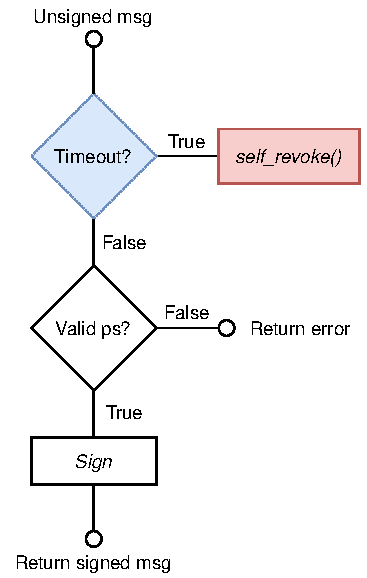
\includegraphics[width=\columnwidth]{figures/drawio/flowchart-sign.drawio.pdf}
    \end{subfigure}
    \unskip\ \vrule\
    \begin{subfigure}[T]{.4\columnwidth}
        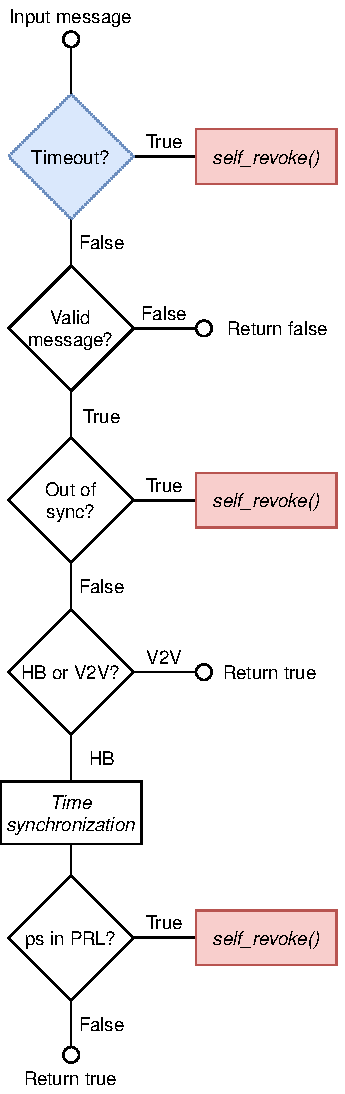
\includegraphics[width=\columnwidth]{figures/drawio/flowchart-process.drawio.pdf}
    \end{subfigure}
    \begin{minipage}{.45\columnwidth}
        \leavevmode\subcaption{Receiving a sign request.}
        \label{fig:appendix:flowchart-sign}
    \end{minipage}\hfil
    \begin{minipage}{.45\columnwidth}
        \leavevmode\subcaption{Receiving a message.}
        \label{fig:appendix:flowchart-process}
    \end{minipage}
    \caption{Flowcharts of the \acs{TC} logic. Blue (dotted) nodes are only
    relevant when a local trusted time source is available in \acsp{TC}.}
    \label{fig:appendix:flowchart}
\end{figure}

%Table~\ref{tbl:eval-variables} describes all variables used in the main paper
%for the reader's convenience. 
\cref{fig:appendix:flowchart} depicts flowcharts for the \ac{TC} behavior
described in our design. In particular, \cref{fig:appendix:flowchart-sign}
illustrates the steps taken to sign a \ac{V2V} message, while
\cref{fig:appendix:flowchart-process} shows the logic to verify a network
message, which can be either a \ac{HB} or a \ac{V2V} message.

According to \cref{req:v2v-receive,eq:valid-v2v-generic,eq:valid-heartbeat},
external messages should be verified with respect to authenticity (via digital
signature verification) and freshness (according to the validity window
\paramtt). Furthermore, the \ac{TC} should automatically perform self-revocation
if it detects de-synchronization (\cref{eq:auto-rev}). For every valid \ac{HB},
the \ac{TC} should synchronize its internal time \funcnow{}
((\cref{eq:time-update}), redundant if a local trusted time source is used), and
then inspect the \ac{PRL} to check whether self-revocation should be executed or
not (\cref{eq:self-rev}). For signing a message, the \ac{TC} should possess
valid pseudonyms in order to make a signature, which includes the input message
and context metadata such as timestamps (\cref{req:v2v-send}).

In \cref{fig:appendix:flowchart}, the \emph{timeout} condition in blue only
applies to the extension that takes into account a local trusted time source in
\ac{TC}, and checks if the current time is bigger than the biggest timestamp
received in a \ac{HB} plus \paramtt{} (\cref{eq:auto-rev-timeout}).
\section{Tamarin Models}
\label{appendix:tamarin}

This appendix extends \cref{section:design-verification}, providing more details
on how we translated our design to \tamarin{} and how we captured the properties
of our design. Here, we also discuss our variant where a trusted time source in
the \ac{TC} is available (cf.~\cref{section:design-extensions}).

\subsection{Mapping our Design to \tamarin{}}

To map our design to Tamarin, we used only six main rules:
%
\begin{itemize}
    \item \tamrule{RA\_generate\_heartbeat}: This rule takes as input the
    current time and \ac{PRL} and produces a new \ac{HB} as output, signed
    with the \ac{RA}'s private key. The \ac{HB} is also sent out to the network
    channel, and an action fact \tamrule{HeartbeatGenerated(HB)} is produced.
    This rule can only be executed once per \ac{PRL} and time step to reduce
    the number of states, since multiple execution with the same parameters
    would generate the same \ac{HB}, which is not relevant in our model since
    \tamarin{} already allows replays of network messages.
    \item \tamrule{RA\_issue\_revocation}: Taking as input the current
    time, \ac{PRL}, and a pseudonym's public key, this rule generates a
    new \ac{PRL} by adding the pseudonym to the list and incrementing the
    sequence number by one. We added a restriction to revoke each pseudonym only
    once. After execution, the action fact \tamrule{RevocationIssued(ps, t)} is
    generated.
    \item \tamrule{TC\_get\_pseudonym}: This rule allows the \ac{TC} to obtain a
    new pseudonym credential. How exactly this credential is obtained (e.g., via
    a communication to the infrastructure) is outside of our scope; What is
    important in our model is that the \ac{TC} can obtain and use an arbitrary
    number of pseudonyms. The only restriction of this rule is to ensure that
    only non-revoked \acp{TC} can obtain new pseudonyms
    (cf.~\cref{req:pseudonym}).
    \item \tamrule{TC\_process\_heartbeat}: The \ac{TC} processes a \ac{HB}
    taken as input from the channel. Restrictions ensure that the received
    \ac{HB} has a valid signature and timestamp. In addition, the \ac{TC} has to
    check whether to perform self-revocation or not. To do so, we divided this
    rule in two mutually-exclusive rules that produce different results: if any
    of the \ac{TC} pseudonyms is in the \ac{PRL}, the action fact
    \tamrule{Revoked(t)} is produced, otherwise it is not. Either way, a
    \tamrule{HeartbeatProcessed(HB,t)} action fact are produced, along with a
    new \tamrule{!Time(t\_hb)} persistent fact to synchronize the \ac{TC} time.
    \item \tamrule{TC\_sign\_message}: The \ac{TC} generates a new \ac{V2V}
    message signed with a pseudonym's private key. It takes the latest time as
    input, while restrictions ensure that the TC has not been previously revoked
    (i.e., the \tamrule{Revoked(t)} action fact does not exist). The rule
    produces a signed timestamped message and sends it to the out channel. A
    \tamrule{Signed(msg,ps)} action fact is produced as well.
    \item \tamrule{process\_message}: This rule models a generic third entity
    that receives a \ac{V2V} message from network and verifies it. If the
    signature is valid and the message is fresh, a
    \tamrule{MessageAccepted(msg,ps,t)} action fact is generated.
\end{itemize}

\subsection{Trusted Time Source in \acp{TC}}

\begin{figure}
  \centering
    \lstinputlisting[language=Tamarin]{properties-time.spthy}
  \caption{Properties of our design with a trusted time source in \ac{TC}
  translated to \tamarin{} lemmas.}
  \label{listing:tamarin-lemmas-time}
\end{figure}

The design that models a trusted time source in \ac{TC} comes with a major
difference, i.e., that \ac{TC} and \ac{RA} use the same \tamrule{!Time} facts.
That is, this means that their clock is perfectly synchronized, and the \ac{TC}
does not need to process \acp{HB} to advance its internal time.

Table~\ref{tbl:tamarin-lemmas-trusted-time} provides the full list of lemmas
used in this variant, most of which are analogous to the main model. The main
difference is that we added three \emph{reusable lemmas}, i.e., lemmas that
\tamarin{} can leverage to prove other lemmas. This was helpful since we
experienced that the two proof lemmas were harder to verify efficiently than in
our main model. By defining additional lemmas marked as \tamrule{reuse}, we
could instead build efficient proofs, allowing \tamarin{} to terminate in only a
few minutes.


\cref{listing:tamarin-lemmas-time} shows the proof properties of this model. Two
are the main differences compared to the main model: First, the
\tamrule{effective\_revocation} lemma can now directly prove our first property
to calculate the exact value for \paramteff. Indeed, we now assume that all
\acp{TC} are perfectly synchronized with the \ac{RA} time, hence the revocation
time is now absolute and comes at $\paramtrev + 2\paramtt$. Second, thanks to
internal timeouts in \ac{TC}, we can have a stronger proof for the second
property, saying that not only does the \ac{TC} not process \acp{HB} generated
after $\paramtrev{} + \paramtt{}$, but also that the \ac{TC} cannot perform
\emph{any} operations after that time because the automatic revocation timeout
would be triggered. To prove this, we defined an additional rule called
\tamrule{TC\_do\_operation}, which models a generic operation performed by the
\ac{TC} via the \tamrule{NewOperation(t)} action fact. This is then used in
\tamrule{no\_operations\_after\_timeout} to prove that there cannot be
\tamrule{NewOperation(t)} action facts with a value for $t$ bigger than
$\paramtrev + \paramtt$.

\begin{table*}
    \renewcommand{\arraystretch}{1.2}
    \newcolumntype{L}{>{\raggedright\arraybackslash}X}
      \centering
      \begin{tabularx}{.97\linewidth}{ | l | c | c | c | L | }
        \hline
        Lemma                                                     & Type   &  Oracle      & Steps & Description  \\
        \hline
        \hline
        \tamrule{sign\_possible}                                  & S      &              & 6     & Ensures that the \ac{TC} can sign \ac{V2V} messages \\
        \hline
        \tamrule{generate\_hb\_possible}                          & S      &              & 5     & Ensures that the \ac{RA} can generate and distribute \acp{HB} \\
        \hline
        \tamrule{issue\_revocation\_possible}                     & S      &              & 5     & Ensures that the \ac{RA} can revoke pseudonyms, adding them to the \ac{PRL} \\
        \hline
        \tamrule{processing\_hb\_possible}                        & S      &              & 9     & Ensures that the \ac{TC} can receive and process a \ac{HB} \\
        \hline
        \tamrule{revocation\_possible}                            & S      &              & 13    & Ensures that the \ac{TC} can self-revoke when receiving a \ac{HB} \\
        \hline
        \tamrule{process\_message\_possible}                      & S      &              & 7     & Ensures that a third entity can process \ac{V2V} messages signed by the \ac{TC}  \\
        \hline
        \tamrule{exists\_par\_tv\_2}                              & S      &              & 5     & Used to verify that \paramtt{} is arbitrary \\
        \hline
        \tamrule{exists\_par\_tv\_4}                              & S      &              & 7     & Used to verify that \paramtt{} is arbitrary \\
        \hline
        \tamrule{no\_signing\_after\_timeout}                     & F      &              & 205   & Ensures that the \ac{TC} cannot make signatures after performing automatic revocation \\
        \hline
        \tamrule{no\_signing\_after\_revocation}                  & F      &              & 2     & Ensures that the \ac{TC} cannot make signatures after performing self-revocation \\
        \hline
        \tamrule{all\_heartbeats\_processed\_within\_tolerance}   & F      & \faCheck     & 260   & Ensures that outdated \ac{HB} are correctly discarded by the \ac{TC} \\
        \hline
        \tamrule{all\_messages\_accepted\_signed\_exists}         & R      & \faCheck     & 62    & Ensures that, for each \ac{V2V} message verified by a third entity, the same message was previously signed by the \ac{TC} \\
        \hline
        \tamrule{all\_messages\_accepted\_within\_tolerance}      & R      & \faCheck     & 282   & Ensures that outdated \ac{V2V} messages are correctly discarded by the third entity \\
        \hline
        \tamrule{no\_messages\_accepted\_after\_revocation}       & R      & \faCheck     & 74    & Ensures that, if revocation is mandated at time \paramtrev, all TC messages accepted by a third entity cannot contain timestamp greater than $\paramtrev{} + \paramtt{}$ \\
        \hline
        \tamrule{effective\_revocation}                           & P      & \faCheck     & 4     & Verifies property \ref{property:revoke} in \cref{section:design-properties} \\
        \hline
        \tamrule{no\_operations\_after\_timeout}                  & P      & \faCheck     & 76    & Verifies property \ref{property:prl} in \cref{section:design-properties} \\
        \hline
      \end{tabularx}
      \vspace{0.2cm}
      \caption{Full list of lemmas proven with \tamarin{} on our model with
      trusted time. \emph{Type} is either \emph{S} (sanity), \emph{F}
      (functional), \emph{R} (reuse) or \emph{P} (proof). \emph{Oracle}
      indicates whether an oracle was needed, while \emph{Steps} the number of
      steps required by \tamarin{} to prove the lemma.}
      \label{tbl:tamarin-lemmas-trusted-time}
      %\vspace{-5mm}
    \end{table*}
    %



\section{Complete Simulation Results}
\label{appendix:simulation}

\begin{table}
\renewcommand{\arraystretch}{1.2}
  \centering
  \begin{tabular}{ | c | c | c | c | c | }
    \hline
    Scenario        & Time? &  \paramtt{} (s)   & \paramteff{} (s)   & \paramtprl{} (s)  \\
    \hline
    \hline
    A1              & no                  & 30                & 60                 & 30                \\
    \hline
    A2              & no                  & 150               & 300                & 150               \\
    \hline
    B1              & yes                 & 30                & 60                 & 30                \\
    \hline
    B2              & yes                 & 150               & 300                & 150               \\
    \hline
  \end{tabular}
  \vspace{0.2cm}
  \caption{ Scenarios evaluated in our simulation. Parameters are chosen
  according to the desired \paramteff{}. The column named \emph{Time?} indicates
  whether a local trusted time source is used in \acp{TC} or not.}
  \label{tbl:eval-scenarios}
  %\vspace{-5mm}
\end{table}
%




\begin{figure}[t]
    %\centering
    \hspace*{-0.3cm}
    \resizebox{1.05\linewidth}{!} {
      % This file was created with tikzplotlib v0.10.1.
\begin{tikzpicture}

\definecolor{chocolate1869726}{RGB}{186,97,26}
\definecolor{darkgoldenrod19413532}{RGB}{194,135,32}
\definecolor{darkslategray38}{RGB}{38,38,38}
\definecolor{darkslategray48}{RGB}{48,48,48}
\definecolor{lavender234234242}{RGB}{234,234,242}
\definecolor{seagreen21138106}{RGB}{21,138,106}
\definecolor{teal23108155}{RGB}{23,108,155}

\begin{axis}[
clip=false,
axis background/.style={fill=lavender234234242},
axis line style={white},
height=8cm,
minor xtick={},
minor ytick={},
tick align=outside,
width=15cm,
x grid style={white},
xlabel=\textcolor{darkslategray38}{Time (s)},
xmajorgrids,
xmajorticks=true,
xmin=-3, xmax=63,
xtick style={color=darkslategray38,draw=none},
xtick={-10,0,10,20,30,40,50,60,70},
y dir=reverse,
y grid style={white},
ymajorticks=true,
ymin=-0.5, ymax=3.5,
ytick style={color=darkslategray38,draw=none},
ytick={0,1,2,3},
yticklabel style={rotate=90.0,anchor=center,yshift=8pt},
yticklabels={honest,smart,blind,smart-prl}
]
% START VERTICAL LINES %
\addplot [dashdotted, black]
table {%
0 3.5
0 -0.5
};
\addplot [dashdotted, gray!60]
table {%
30 3.5
30 -0.5
};
\addplot [dashdotted, black]
table {%
60 3.5
60 -0.5
};
% END VERTICAL LINES %
\path [draw=darkslategray48, fill=teal23108155, semithick]
(axis cs:11.5,-0.4)
--(axis cs:11.5,0.4)
--(axis cs:23,0.4)
--(axis cs:23,-0.4)
--(axis cs:11.5,-0.4)
--cycle;
\path [draw=darkslategray48, fill=darkgoldenrod19413532, semithick]
(axis cs:30,0.6)
--(axis cs:30,1.4)
--(axis cs:34,1.4)
--(axis cs:34,0.6)
--(axis cs:30,0.6)
--cycle;
\path [draw=darkslategray48, fill=seagreen21138106, semithick]
(axis cs:15,1.6)
--(axis cs:15,2.4)
--(axis cs:25,2.4)
--(axis cs:25,1.6)
--(axis cs:15,1.6)
--cycle;
\path [draw=darkslategray48, fill=chocolate1869726, semithick]
(axis cs:15,2.6)
--(axis cs:15,3.4)
--(axis cs:24,3.4)
--(axis cs:24,2.6)
--(axis cs:15,2.6)
--cycle;
\addplot [semithick, darkslategray48]
table {%
11.5 0
1 0
};
\addplot [semithick, darkslategray48]
table {%
23 0
38 0
};
\addplot [semithick, darkslategray48]
table {%
1 -0.2
1 0.2
};
\addplot [semithick, darkslategray48]
table {%
38 -0.2
38 0.2
};
\addplot [semithick, darkslategray48]
table {%
30 1
24 1
};
\addplot [semithick, darkslategray48]
table {%
34 1
40 1
};
\addplot [semithick, darkslategray48]
table {%
24 0.8
24 1.2
};
\addplot [semithick, darkslategray48]
table {%
40 0.8
40 1.2
};
\addplot [black, mark=diamond*, mark size=1.5, mark options={solid,fill=darkslategray48}, only marks]
table {%
2 1
23 1
10 1
18 1
14 1
4 1
8 1
17 1
21 1
44 1
43 1
41 1
42 1
41 1
42 1
43 1
41 1
43 1
42 1
42 1
};
\addplot [semithick, darkslategray48]
table {%
15 2
3 2
};
\addplot [semithick, darkslategray48]
table {%
25 2
33 2
};
\addplot [semithick, darkslategray48]
table {%
3 1.8
3 2.2
};
\addplot [semithick, darkslategray48]
table {%
33 1.8
33 2.2
};
\addplot [semithick, darkslategray48]
table {%
15 3
2 3
};
\addplot [semithick, darkslategray48]
table {%
24 3
35 3
};
\addplot [semithick, darkslategray48]
table {%
2 2.8
2 3.2
};
\addplot [semithick, darkslategray48]
table {%
35 2.8
35 3.2
};
\addplot [black, mark=diamond*, mark size=1.5, mark options={solid,fill=darkslategray48}, only marks]
table {%
1 3
1 3
};
\addplot [semithick, darkslategray48]
table {%
17 -0.4
17 0.4
};
\addplot [semithick, darkslategray48]
table {%
32 0.6
32 1.4
};
\addplot [semithick, darkslategray48]
table {%
20 1.6
20 2.4
};
\addplot [semithick, darkslategray48]
table {%
20 2.6
20 3.4
};
\draw (axis cs:-3.5,-0.58) node[
  scale=1,
  anchor=base west,
  text=darkslategray38,
  rotate=0.0
]{\textsc{Revoke}};
\draw[dashed] (axis cs:29,-0.58) node[
  scale=1,
  anchor=base west,
  text=darkslategray38,
  rotate=0.0
]{$T_{\mathsf{v}}$};
\draw (axis cs:58.5,-0.58) node[
  scale=1,
  anchor=base west,
  text=darkslategray38,
  rotate=0.0
]{$T_{\mathsf{eff}}$};
\end{axis}

\end{tikzpicture}

    } \caption{Simulation results for scenario A1.}
    \label{fig:eval-sim-a1}
\end{figure}

\begin{figure}[t]
    %\centering
    \hspace*{-0.3cm}
    \resizebox{1.05\linewidth}{!} {
      % This file was created with tikzplotlib v0.10.1.
\begin{tikzpicture}

\definecolor{chocolate1869726}{RGB}{186,97,26}
\definecolor{darkgoldenrod19413532}{RGB}{194,135,32}
\definecolor{darkslategray38}{RGB}{38,38,38}
\definecolor{darkslategray48}{RGB}{48,48,48}
\definecolor{lavender234234242}{RGB}{234,234,242}
\definecolor{seagreen21138106}{RGB}{21,138,106}
\definecolor{teal23108155}{RGB}{23,108,155}

\begin{axis}[
clip=false,
axis background/.style={fill=lavender234234242},
axis line style={white},
height=8cm,
minor xtick={},
minor ytick={},
tick align=outside,
width=15cm,
x grid style={white},
xlabel=\textcolor{darkslategray38}{Time (s)},
xmajorgrids,
xmajorticks=true,
xmin=-15, xmax=315,
xtick style={color=darkslategray38,draw=none},
xtick={-50,0,50,100,150,200,250,300,350},
y dir=reverse,
y grid style={white},
ymajorticks=true,
ymin=-0.5, ymax=3.5,
ytick style={color=darkslategray38,draw=none},
ytick={0,1,2,3},
yticklabel style={rotate=90.0,anchor=center,yshift=8pt},
yticklabels={honest,smart,blind,smart-prl}
]
% START VERTICAL LINES %
\addplot [dashdotted, black]
table {%
0 3.5
0 -0.5
};
\addplot [dashdotted, gray!60]
table {%
150 3.5
150 -0.5
};
\addplot [dashdotted, black]
table {%
300 3.5
300 -0.5
};
% END VERTICAL LINES %
\path [draw=darkslategray48, fill=teal23108155, semithick]
(axis cs:103,-0.4)
--(axis cs:103,0.4)
--(axis cs:131,0.4)
--(axis cs:131,-0.4)
--(axis cs:103,-0.4)
--cycle;
\path [draw=darkslategray48, fill=darkgoldenrod19413532, semithick]
(axis cs:150,0.6)
--(axis cs:150,1.4)
--(axis cs:155,1.4)
--(axis cs:155,0.6)
--(axis cs:150,0.6)
--cycle;
\path [draw=darkslategray48, fill=seagreen21138106, semithick]
(axis cs:29.75,1.6)
--(axis cs:29.75,2.4)
--(axis cs:125.25,2.4)
--(axis cs:125.25,1.6)
--(axis cs:29.75,1.6)
--cycle;
\path [draw=darkslategray48, fill=chocolate1869726, semithick]
(axis cs:111,2.6)
--(axis cs:111,3.4)
--(axis cs:136,3.4)
--(axis cs:136,2.6)
--(axis cs:111,2.6)
--cycle;
\addplot [semithick, darkslategray48]
table {%
103 0
62 0
};
\addplot [semithick, darkslategray48]
table {%
131 0
162 0
};
\addplot [semithick, darkslategray48]
table {%
62 -0.2
62 0.2
};
\addplot [semithick, darkslategray48]
table {%
162 -0.2
162 0.2
};
\addplot [black, mark=diamond*, mark size=1.5, mark options={solid,fill=darkslategray48}, only marks]
table {%
4 0
15 0
31 0
33 0
4 0
37 0
25 0
47 0
28 0
54 0
23 0
54 0
46 0
54 0
};
\addplot [semithick, darkslategray48]
table {%
150 1
145 1
};
\addplot [semithick, darkslategray48]
table {%
155 1
162 1
};
\addplot [semithick, darkslategray48]
table {%
145 0.8
145 1.2
};
\addplot [semithick, darkslategray48]
table {%
162 0.8
162 1.2
};
\addplot [black, mark=diamond*, mark size=1.5, mark options={solid,fill=darkslategray48}, only marks]
table {%
127 1
73 1
89 1
96 1
84 1
118 1
80 1
134 1
28 1
79 1
120 1
127 1
120 1
51 1
130 1
65 1
88 1
71 1
112 1
68 1
27 1
73 1
79 1
44 1
74 1
1 1
121 1
6 1
95 1
92 1
139 1
70 1
138 1
11 1
167 1
166 1
169 1
163 1
170 1
167 1
167 1
169 1
168 1
167 1
167 1
166 1
163 1
171 1
165 1
};
\addplot [semithick, darkslategray48]
table {%
29.75 2
2 2
};
\addplot [semithick, darkslategray48]
table {%
125.25 2
159 2
};
\addplot [semithick, darkslategray48]
table {%
2 1.8
2 2.2
};
\addplot [semithick, darkslategray48]
table {%
159 1.8
159 2.2
};
\addplot [semithick, darkslategray48]
table {%
111 3
74 3
};
\addplot [semithick, darkslategray48]
table {%
136 3
154 3
};
\addplot [semithick, darkslategray48]
table {%
74 2.8
74 3.2
};
\addplot [semithick, darkslategray48]
table {%
154 2.8
154 3.2
};
\addplot [black, mark=diamond*, mark size=1.5, mark options={solid,fill=darkslategray48}, only marks]
table {%
1 3
61 3
27 3
40 3
27 3
2 3
64 3
49 3
67 3
19 3
2 3
2 3
10 3
31 3
39 3
66 3
33 3
40 3
41 3
39 3
49 3
5 3
};
\addplot [semithick, darkslategray48]
table {%
117 -0.4
117 0.4
};
\addplot [semithick, darkslategray48]
table {%
152 0.6
152 1.4
};
\addplot [semithick, darkslategray48]
table {%
79.5 1.6
79.5 2.4
};
\addplot [semithick, darkslategray48]
table {%
126 2.6
126 3.4
};
\draw (axis cs:-17.5,-0.58) node[
  scale=1,
  anchor=base west,
  text=darkslategray38,
  rotate=0.0
]{\textsc{Revoke}};
\draw[dashed] (axis cs:143,-0.58) node[
  scale=1,
  anchor=base west,
  text=darkslategray38,
  rotate=0.0
]{$T_{\mathsf{v}}$};
\draw (axis cs:292,-0.58) node[
  scale=1,
  anchor=base west,
  text=darkslategray38,
  rotate=0.0
]{$T_{\mathsf{eff}}$};
\end{axis}

\end{tikzpicture}

    } \caption{Simulation results for scenario A2.}
    \label{fig:eval-sim-a2}
\end{figure}

\begin{figure}[t]
    %\centering
    \hspace*{-0.3cm}
    \resizebox{1.05\linewidth}{!} {
      % This file was created with tikzplotlib v0.10.1.
\begin{tikzpicture}

\definecolor{chocolate1869726}{RGB}{186,97,26}
\definecolor{darkgoldenrod19413532}{RGB}{194,135,32}
\definecolor{darkslategray38}{RGB}{38,38,38}
\definecolor{darkslategray48}{RGB}{48,48,48}
\definecolor{lavender234234242}{RGB}{234,234,242}
\definecolor{seagreen21138106}{RGB}{21,138,106}
\definecolor{teal23108155}{RGB}{23,108,155}

\begin{axis}[
clip=false,
axis background/.style={fill=lavender234234242},
axis line style={white},
height=8cm,
minor xtick={},
minor ytick={},
tick align=outside,
width=15cm,
x grid style={white},
xlabel=\textcolor{darkslategray38}{Time (s)},
xmajorgrids,
xmajorticks=true,
xmin=-1.9, xmax=61.9,
xtick style={color=darkslategray38,draw=none},
xtick={-10,0,10,20,30,40,50,60,70},
y dir=reverse,
y grid style={white},
ymajorticks=true,
ymin=-0.5, ymax=3.5,
ytick style={color=darkslategray38,draw=none},
ytick={0,1,2,3},
yticklabel style={rotate=90.0,anchor=center,yshift=8pt},
yticklabels={honest,smart,blind,smart-prl}
]
% START VERTICAL LINES %
\addplot [dashdotted, black]
table {%
0 3.5
0 -0.5
};
\addplot [dashdotted, gray!60]
table {%
30 3.5
30 -0.5
};
\addplot [dashdotted, black]
table {%
60 3.5
60 -0.5
};
% END VERTICAL LINES %
\path [draw=darkslategray48, fill=teal23108155, semithick]
(axis cs:12,-0.4)
--(axis cs:12,0.4)
--(axis cs:25,0.4)
--(axis cs:25,-0.4)
--(axis cs:12,-0.4)
--cycle;
\path [draw=darkslategray48, fill=darkgoldenrod19413532, semithick]
(axis cs:37,0.6)
--(axis cs:37,1.4)
--(axis cs:50,1.4)
--(axis cs:50,0.6)
--(axis cs:37,0.6)
--cycle;
\path [draw=darkslategray48, fill=seagreen21138106, semithick]
(axis cs:16,1.6)
--(axis cs:16,2.4)
--(axis cs:40.5,2.4)
--(axis cs:40.5,1.6)
--(axis cs:16,1.6)
--cycle;
\path [draw=darkslategray48, fill=chocolate1869726, semithick]
(axis cs:13,2.6)
--(axis cs:13,3.4)
--(axis cs:23,3.4)
--(axis cs:23,2.6)
--(axis cs:13,2.6)
--cycle;
\addplot [semithick, darkslategray48]
table {%
12 0
1 0
};
\addplot [semithick, darkslategray48]
table {%
25 0
38 0
};
\addplot [semithick, darkslategray48]
table {%
1 -0.2
1 0.2
};
\addplot [semithick, darkslategray48]
table {%
38 -0.2
38 0.2
};
\addplot [semithick, darkslategray48]
table {%
37 1
19 1
};
\addplot [semithick, darkslategray48]
table {%
50 1
59 1
};
\addplot [semithick, darkslategray48]
table {%
19 0.8
19 1.2
};
\addplot [semithick, darkslategray48]
table {%
59 0.8
59 1.2
};
\addplot [black, mark=diamond*, mark size=1.5, mark options={solid,fill=darkslategray48}, only marks]
table {%
2 1
5 1
16 1
14 1
};
\addplot [semithick, darkslategray48]
table {%
16 2
3 2
};
\addplot [semithick, darkslategray48]
table {%
40.5 2
50 2
};
\addplot [semithick, darkslategray48]
table {%
3 1.8
3 2.2
};
\addplot [semithick, darkslategray48]
table {%
50 1.8
50 2.2
};
\addplot [semithick, darkslategray48]
table {%
13 3
1 3
};
\addplot [semithick, darkslategray48]
table {%
23 3
37 3
};
\addplot [semithick, darkslategray48]
table {%
1 2.8
1 3.2
};
\addplot [semithick, darkslategray48]
table {%
37 2.8
37 3.2
};
\addplot [black, mark=diamond*, mark size=1.5, mark options={solid,fill=darkslategray48}, only marks]
table {%
49 3
};
\addplot [semithick, darkslategray48]
table {%
20 -0.4
20 0.4
};
\addplot [semithick, darkslategray48]
table {%
43 0.6
43 1.4
};
\addplot [semithick, darkslategray48]
table {%
31 1.6
31 2.4
};
\addplot [semithick, darkslategray48]
table {%
18 2.6
18 3.4
};
\draw (axis cs:-3.5,-0.58) node[
  scale=1,
  anchor=base west,
  text=darkslategray38,
  rotate=0.0
]{\textsc{Revoke}};
\draw[dashed] (axis cs:29,-0.58) node[
  scale=1,
  anchor=base west,
  text=darkslategray38,
  rotate=0.0
]{$T_{\mathsf{v}}$};
\draw (axis cs:58.5,-0.58) node[
  scale=1,
  anchor=base west,
  text=darkslategray38,
  rotate=0.0
]{$T_{\mathsf{eff}}$};
\end{axis}

\end{tikzpicture}

    } \caption{Simulation results for scenario B1.}
    \label{fig:eval-sim-b1}
\end{figure}

\begin{figure}[t]
    %\centering
    \hspace*{-0.3cm}
    \resizebox{1.05\linewidth}{!} {
      % This file was created with tikzplotlib v0.10.1.
\begin{tikzpicture}

\definecolor{chocolate1869726}{RGB}{186,97,26}
\definecolor{darkgoldenrod19413532}{RGB}{194,135,32}
\definecolor{darkslategray38}{RGB}{38,38,38}
\definecolor{darkslategray48}{RGB}{48,48,48}
\definecolor{lavender234234242}{RGB}{234,234,242}
\definecolor{seagreen21138106}{RGB}{21,138,106}
\definecolor{teal23108155}{RGB}{23,108,155}

\begin{axis}[
clip=false,
axis background/.style={fill=lavender234234242},
axis line style={white},
height=8cm,
minor xtick={},
minor ytick={},
tick align=outside,
width=15cm,
x grid style={white},
xlabel=\textcolor{darkslategray38}{Time (s)},
xmajorgrids,
xmajorticks=true,
xmin=-13.85, xmax=312.85,
xtick style={color=darkslategray38,draw=none},
xtick={-50,0,50,100,150,200,250,300,350},
y dir=reverse,
y grid style={white},
ymajorticks=true,
ymin=-0.5, ymax=3.5,
ytick style={color=darkslategray38,draw=none},
ytick={0,1,2,3},
yticklabel style={rotate=90.0,anchor=center,yshift=8pt},
yticklabels={honest,smart,blind,smart-prl}
]
% START VERTICAL LINES %
\addplot [dashdotted, black]
table {%
0 3.5
0 -0.5
};
\addplot [dashdotted, gray!60]
table {%
150 3.5
150 -0.5
};
\addplot [dashdotted, black]
table {%
300 3.5
300 -0.5
};
% END VERTICAL LINES %
\path [draw=darkslategray48, fill=teal23108155, semithick]
(axis cs:104,-0.4)
--(axis cs:104,0.4)
--(axis cs:135,0.4)
--(axis cs:135,-0.4)
--(axis cs:104,-0.4)
--cycle;
\path [draw=darkslategray48, fill=darkgoldenrod19413532, semithick]
(axis cs:240,0.6)
--(axis cs:240,1.4)
--(axis cs:274,1.4)
--(axis cs:274,0.6)
--(axis cs:240,0.6)
--cycle;
\path [draw=darkslategray48, fill=seagreen21138106, semithick]
(axis cs:91.25,1.6)
--(axis cs:91.25,2.4)
--(axis cs:220.25,2.4)
--(axis cs:220.25,1.6)
--(axis cs:91.25,1.6)
--cycle;
\path [draw=darkslategray48, fill=chocolate1869726, semithick]
(axis cs:108,2.6)
--(axis cs:108,3.4)
--(axis cs:140,3.4)
--(axis cs:140,2.6)
--(axis cs:108,2.6)
--cycle;
\addplot [semithick, darkslategray48]
table {%
104 0
61 0
};
\addplot [semithick, darkslategray48]
table {%
135 0
160 0
};
\addplot [semithick, darkslategray48]
table {%
61 -0.2
61 0.2
};
\addplot [semithick, darkslategray48]
table {%
160 -0.2
160 0.2
};
\addplot [black, mark=diamond*, mark size=1.5, mark options={solid,fill=darkslategray48}, only marks]
table {%
3 0
26 0
48 0
7 0
19 0
15 0
47 0
31 0
6 0
9 0
20 0
39 0
47 0
34 0
26 0
43 0
24 0
56 0
44 0
14 0
16 0
21 0
23 0
16 0
};
\addplot [semithick, darkslategray48]
table {%
240 1
190 1
};
\addplot [semithick, darkslategray48]
table {%
274 1
298 1
};
\addplot [semithick, darkslategray48]
table {%
190 0.8
190 1.2
};
\addplot [semithick, darkslategray48]
table {%
298 0.8
298 1.2
};
\addplot [black, mark=diamond*, mark size=1.5, mark options={solid,fill=darkslategray48}, only marks]
table {%
135 1
127 1
3 1
68 1
90 1
180 1
113 1
149 1
123 1
186 1
83 1
180 1
146 1
137 1
166 1
8 1
7 1
78 1
3 1
160 1
28 1
64 1
22 1
68 1
125 1
47 1
172 1
140 1
36 1
55 1
148 1
80 1
171 1
145 1
3 1
102 1
14 1
184 1
18 1
34 1
100 1
84 1
11 1
142 1
131 1
83 1
37 1
135 1
167 1
};
\addplot [semithick, darkslategray48]
table {%
91.25 2
1 2
};
\addplot [semithick, darkslategray48]
table {%
220.25 2
285 2
};
\addplot [semithick, darkslategray48]
table {%
1 1.8
1 2.2
};
\addplot [semithick, darkslategray48]
table {%
285 1.8
285 2.2
};
\addplot [semithick, darkslategray48]
table {%
108 3
61 3
};
\addplot [semithick, darkslategray48]
table {%
140 3
188 3
};
\addplot [semithick, darkslategray48]
table {%
61 2.8
61 3.2
};
\addplot [semithick, darkslategray48]
table {%
188 2.8
188 3.2
};
\addplot [black, mark=diamond*, mark size=1.5, mark options={solid,fill=darkslategray48}, only marks]
table {%
42 3
57 3
31 3
3 3
5 3
22 3
26 3
13 3
5 3
18 3
58 3
1 3
3 3
41 3
4 3
24 3
42 3
55 3
57 3
38 3
53 3
15 3
52 3
37 3
276 3
202 3
222 3
229 3
195 3
219 3
194 3
193 3
264 3
266 3
236 3
207 3
200 3
226 3
259 3
247 3
203 3
204 3
243 3
248 3
239 3
288 3
197 3
252 3
255 3
190 3
};
\addplot [semithick, darkslategray48]
table {%
121 -0.4
121 0.4
};
\addplot [semithick, darkslategray48]
table {%
260 0.6
260 1.4
};
\addplot [semithick, darkslategray48]
table {%
148 1.6
148 2.4
};
\addplot [semithick, darkslategray48]
table {%
125 2.6
125 3.4
};
\draw (axis cs:-17.5,-0.58) node[
  scale=1,
  anchor=base west,
  text=darkslategray38,
  rotate=0.0
]{\textsc{Revoke}};
\draw[dashed] (axis cs:143,-0.58) node[
  scale=1,
  anchor=base west,
  text=darkslategray38,
  rotate=0.0
]{$T_{\mathsf{v}}$};
\draw (axis cs:292,-0.58) node[
  scale=1,
  anchor=base west,
  text=darkslategray38,
  rotate=0.0
]{$T_{\mathsf{eff}}$};
\end{axis}

\end{tikzpicture}

    } \caption{Simulation results for scenario B2.}
    \label{fig:eval-sim-b2}
\end{figure}

We ran simulations for each of the scenarios described in
\cref{tbl:eval-scenarios}. Results are depicted in
\cref{fig:eval-sim-a1,fig:eval-sim-a2,fig:eval-sim-b1,fig:eval-sim-b2}.

Recall from \cref{section:eval-sim} that each value of the boxes represents the
time between the revocation of \ps{} (\funcrevokedaa{} event) and the last
\ac{V2V} message signed with \ps{} that was verified by a non-malicious \ac{TC}
(\funcverify{} event). The latter time represents the \emph{effective revocation
time} for that particular pseudonym \ps. The box plots give the distribution of
such values, obtained aggregating more than 600 revocations, filtering out
negative values.

The figures show one significant difference between the main design (A1 and A2)
and the extension with a local trusted time source (B1 and B2): While in the
former most revocations are effective around or before \paramtt{}, in the latter
attackers are able to postpone revocation up until \paramteff{} in some cases,
i.e., it appears easier to reach the upper bound, especially for powerful
attackers such as the \attackersmart{} one. This is due to the fact that, while
in the main design revoked \acp{TC} cannot synchronize their time since
\paramtrev, with a local time source \acp{TC} can still advance their internal
time up until $\paramtrev + \paramtt$, before triggering the automatic
revocation logic. That is, in the latter case a revoked \ac{TC} is able to
generate ''more fresh'' \ac{V2V} messages, which can be processed by other
\acp{TC} later in time.

This peculiarity suggests that a local trusted time source negatively affects
the revocation time. While this may be true in the average case, it still does
not affect the worst-case effective revocation time \paramteff, as shown in the
figures.
\section{Calculating Expected Size of the PRL}
\label{appendix:markov}

This appendix covers the basics of the utilized probabilities to then explain
the Markov matrix. We also describe the calculation of the stationary
distribution as a means to calculate the expected \ac{PRL} size. Finally, we
discuss the computation of the probabilities and expected values used in
\cref{section:eval-prl-size}.

\subsection{Utilized Probabilities}

Recall from \cref{section:eval-prl-size} that we model the processes of gaining
and losing pseudonyms from the \ac{PRL} as two individual probabilities, then we
combine them in the next step into a Markov chain. The two probabilities shown
in \cref{eq:prl-size-g} and \cref{eq:prl-size-l} are denoted as $G_{il}$ and
$L_{il}$ respectively and can be seen as probability matrices that at location
$il$ have the probability for being in state $i$ and gaining or losing $l$
pseudonyms from the list. The core assumption for these two probabilities is
that both adding and removing pseudonyms from the revocation list can be seen as
a binomial distribution that only depends on:
\begin{inparaenum}
    \item the current size of the list, i.e., how many certificates there are left to be revoked or removed from the list,
    \item the probability for each pseudonym to be revoked at any given time, and
    \item the time that a pseudonym stays in the list.
\end{inparaenum}
As such, this model assumes that pseudonyms are renewed as soon as they are
evicted from the \ac{PRL}, i.e., the list can never hold more than the total
number of $n$ pseudonyms, which is a realistic assumption for large $n$ as it is
unlikely that so many pseudonyms in the system would be revoked in a short time
during regular operation.  Furthermore, in this way we model the process of
losing pseudonyms from the list as a probabilistic process that has the expected
value at $T_{prl}$.  We, however, can not model a precise eviction of the
pseudonym from the \ac{PRL} after $T_{prl}$ time steps.  In our view this is an
acceptable tradeoff as on average and over the lifetime of the \ac{PRL}, the
modeled behavior comes very close to the actual behavior of evicting pseudonyms
from the \ac{PRL} after exactly $T_{prl}$ time steps.

\subsection{Markov Model}
We can now combine these two probabilities into a matrix that at location
$p_{ij}$ has the probability of moving from state $i$ to state $j$. Starting
with the simple example of $n=3$ pseudonyms, multiple entries of this matrix are
straightforward:
\begin{itemize}
    \item Starting at any state $i$ and stepping into state $j=0$ requires to not revoke any new pseudonyms and to lose all existing pseudonyms from the list. This is the combination of the two probabilities $L_{ii}G_{i0}$. For example, going from state $i=2$ to $j=0$ requires to lose 2 pseudonyms when there are $2$ in the \ac{PRL}, and requires to gain no new pseudonyms when there are already $2$, leading to the two probabilities $L_{22}G_{20}$
    \item Starting at state $i=0$ and stepping into a state $j$ implies that no pseudonyms can be lost from the \ac{PRL} and $j$ pseudonyms have to be added.
    \item Similarly, starting in state $i=3$ and stepping into any state $j$
    implies that no pseudonyms can be gained, but $j-i$ pseudonyms are removed
    from the \ac{PRL}.
\end{itemize}

The most interesting state transitions in this probability matrix are the
transitions that consist of multiple combinations of events. One example is the
transition from $i=2$ to $j=1$. Here, we first have the obvious possibility that
we reach the state $j=1$, i.e., one pseudonym in the \ac{PRL}, by losing one
pseudonym and gaining none. However, we also have the possibility to lose both
pseudonyms in the \ac{PRL} and gain one, leading to still one remaining
pseudonym in the \ac{PRL}. This is because the pseudonyms in the \ac{PRL} and
outside of the \ac{PRL} are independent and pseudonyms can still be revoked
while others are removed from the list. Thus, the state transition consists of
the following parts: $p_{21} = L_{21}G_{20} + L_{22}G_{21}$.

The full state probability matrix for $n=3$ pseudonyms can be seen below. Note
that a matrix for $n$ pseudonyms is a $n+1 \times n+1$ matrix to accommodate the
state of the empty \ac{PRL}.\vspace{2mm}\\
\begin{math}
    P =
    \left[ {\begin{smallmatrix}{}
      L_{00}G_{00} & L_{00}G_{01} & L_{00}G_{02} & L_{00}G_{03} \\
      L_{11}G_{10} & L_{10}G_{10} + L_{11}G_{11} & L_{10}G_{11} + L_{11}G_{12} & L_{10}G_{12} \\
      L_{22}G_{20} & L_{21}G_{20} + L_{22}G_{21} & L_{20}G_{20} + L_{21}G_{21} & L_{20}G_{21} \\
      L_{33}G_{30} & L_{32}G_{30} & L_{31}G_{30} & L_{30}G_{30} \\
    \end{smallmatrix} } \right]
\end{math}
\vspace{2mm}

\begin{figure}
    \centering
    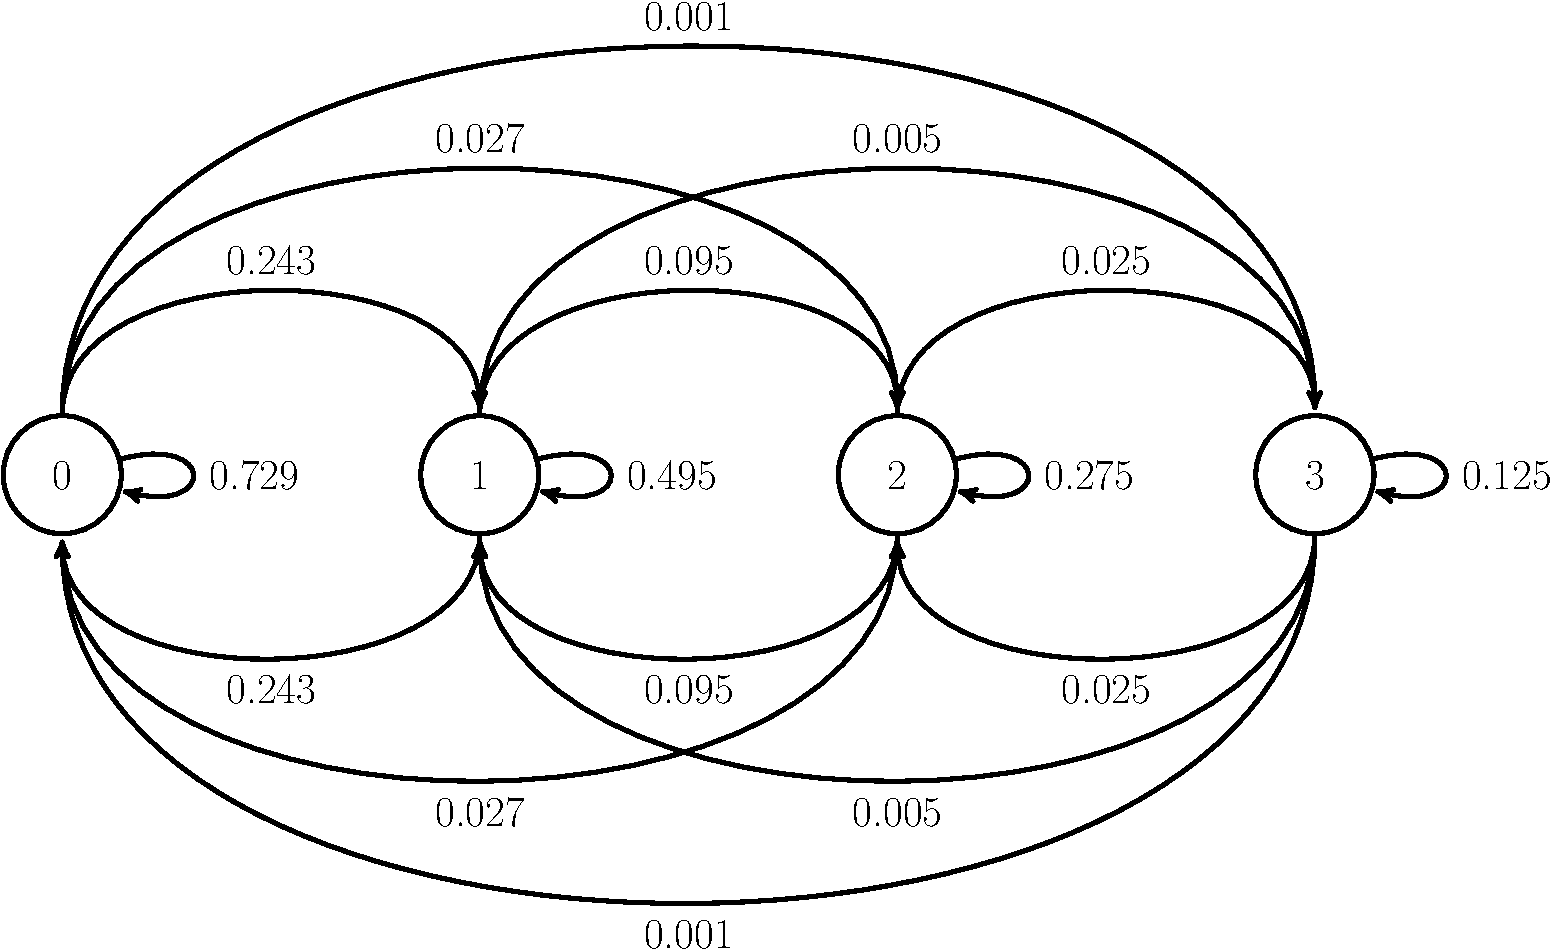
\includegraphics[width=.85\columnwidth]{figures/markov-tikzplot/small-tikz.pdf}
    \caption{A graph of the Markov chain with the exemplary parameters of $n=3$, $p=0.1$, and $T_{prl}=2$.}
    \label{fig:appendix:markov-graph}
\end{figure}

Such probability matrices are also called discrete time Markov
chains~\cite{hermanns2002markov}. \Cref{fig:appendix:markov-graph} depicts the
transition graph for the above Markov chain when we assume the parameters of
$p=0.1$ and $T_{prl}=2$. Based on this first small example, we can approach a
closed formula for an arbitrary number of pseudonyms ($n$). This closed formula
is shown in \cref{eq:prl-size-markov}. The core idea is that each entry depends
on a combination of gaining and losing pseudonyms based on the maximum of $i-j$
and $0$ and ranges up to $i$. Then, any state combination that is not possible
will be $0$ through the binomial coefficient. However, this range is necessary
to catch the complicated combinations in the center of the matrix. Each
combination is then based on losing $l$ pseudonyms from the list and gaining
$l-i+j$ pseudonyms, which basically iterates through the combinations with $l$
as a stepping variable.

\subsection{Calculating the Expected PRL Size}

In discrete time Markov chains, a probability state vector $\pi$ can be multiplied with the Markov matrix $P$ to gain the probabilities for $\pi$ after a single transition in the model~\cite{hermanns2002markov} as follows: $\pi' = \pi \cdot P$.
This, however, is only sufficient to gain the state probabilities after specific amounts of steps.
In contrast to this approach, Markov chains may approach a so-called state equilibrium which is a stationary probability distribution that does not change even after taking a step in the Markov chain.
The stationary distribution follows the equation $\pi = \pi \cdot P$~\cite{hermanns2002markov}.

To gain this stationary distribution, we solve the following equation system:
\begin{flalign*}
                &\pi = \pi P&\\
&\leftrightarrow \pi - \pi P = 0&\\
&\leftrightarrow \pi ( I - P ) = 0&\\
&\leftrightarrow ( I - P )^T \pi^T = 0&
\end{flalign*}

Lastly, since there may be several solutions to this linear equation, we add the
specific constraint to this equation system that the sum of $\pi$ is equal to
$1$. This is the case for each probability vector in Markov
models~\cite{hermanns2002markov}, and follows the intuition that, from any state
probability, the probability to reach any other state is $1$. To add this
constraint, we add a row of $1$ to $( I - P )^T$ and append a $1$ to the zero
vector. Solving this linear equation yields a stationary distribution that is
stable. \cref{fig:eval-prl-size} summarizes this stationary distribution by
showing the list sizes that occur to 75\%, 90\%, and to 99.99\%. The graph shows
these percentiles under different scenarios, i.e., with different shares of
attackers in the network.

\begin{figure}[t]
    \centering
    \resizebox{.83\linewidth}{!}{% changed from auto generated plot:
% width=\columnwidth,
% legend pos=north west,
% and escape the % signs in the labels
% Color order: steelblue88116163 peru20313699 mediumseagreen95157109 indianred1819295
% This file was created with tikzplotlib v0.10.1.
\begin{tikzpicture}

\definecolor{lightgray204}{RGB}{204,204,204}
\definecolor{darkslategray38}{RGB}{38,38,38}
\definecolor{darkslategray76}{RGB}{76,76,76}
\definecolor{indianred1819295}{RGB}{181,92,95}
\definecolor{lavender234234242}{RGB}{234,234,242}
\definecolor{lightslategray133122170}{RGB}{133,122,170}
\definecolor{mediumseagreen95157109}{RGB}{95,157,109}
\definecolor{peru20313699}{RGB}{203,136,99}
\definecolor{steelblue76114176}{RGB}{76,114,176}
\definecolor{steelblue88116163}{RGB}{88,116,163}


\begin{axis}[
width=\columnwidth,
legend pos=north west,
ylabel= PRL size (99th percentile),
xlabel= Number of pseudonyms,
xmajorgrids,
xmajorticks=true,
ymajorgrids,
ymajorticks=true,
axis background/.style={fill=lavender234234242},
axis line style={white},
x grid style={white},
y grid style={white},
legend cell align={left},
legend style={
fill opacity=0.8,
draw opacity=1,
text opacity=1,
at={(0.03,0.97)},
anchor=north west,
draw=lightgray204,
% fill=lavender234234242
},
tick align=outside,
tick pos=left,
xmin=370, xmax=1030,
xtick style={color=black},
ymin=0.0, ymax=15.5,
ytick style={color=black}
]
\addplot [draw=steelblue88116163, fill=steelblue88116163, mark=*, only marks]
table
\addplot [draw=peru20313699, fill=peru20313699, mark=triangle*, only marks]
table
\addplot [draw=mediumseagreen95157109, fill=mediumseagreen95157109, mark=square*, only marks]
table
\addplot [draw=indianred1819295, fill=indianred1819295, mark=diamond*, only marks]
table
\end{axis}

\end{tikzpicture}} 
    \caption{99th percentile PRL sizes for fixed $T_{prl}=30$ and varying number of pseudonyms ($n$) under four scenarios.}
    \label{fig:appendix:markov-n}   
\end{figure}

\begin{figure}[t]
    \centering
    \resizebox{.83\linewidth}{!}{% changed from auto generated plot:
% width=\columnwidth,
% legend pos=north west,
% and escape the % signs in the labels
% Color order: steelblue88116163 peru20313699 mediumseagreen95157109 indianred1819295

% This file was created with tikzplotlib v0.10.1.
\begin{tikzpicture}

\definecolor{lightgray204}{RGB}{204,204,204}
\definecolor{darkslategray38}{RGB}{38,38,38}
\definecolor{darkslategray76}{RGB}{76,76,76}
\definecolor{indianred1819295}{RGB}{181,92,95}
\definecolor{lavender234234242}{RGB}{234,234,242}
\definecolor{lightslategray133122170}{RGB}{133,122,170}
\definecolor{mediumseagreen95157109}{RGB}{95,157,109}
\definecolor{peru20313699}{RGB}{203,136,99}
\definecolor{steelblue76114176}{RGB}{76,114,176}
\definecolor{steelblue88116163}{RGB}{88,116,163}

\begin{axis}[
width=\columnwidth,
legend pos=north west,
ylabel= PRL size (99th percentile),
xlabel= $T_{prl}$,
xmajorgrids,
xmajorticks=true,
ymajorgrids,
ymajorticks=true,
axis background/.style={fill=lavender234234242},
axis line style={white},
x grid style={white},
y grid style={white},
legend cell align={left},
legend style={
fill opacity=0.8,
draw opacity=1,
text opacity=1,
at={(0.03,0.97)},
anchor=north west,
draw=lightgray204
},
tick align=outside,
tick pos=left,
x grid style={white},
xmin=5, xmax=205,
xtick style={color=black},
y grid style={white},
ymin=0.0, ymax=52,
ytick style={color=black}
]
\addplot [draw=steelblue88116163, fill=steelblue88116163, mark=*, only marks]
table
\addplot [draw=peru20313699, fill=peru20313699, mark=triangle*, only marks]
table
\addplot [draw=mediumseagreen95157109, fill=mediumseagreen95157109, mark=square*, only marks]
table
\addplot [draw=indianred1819295, fill=indianred1819295, mark=diamond*, only marks]
table
\end{axis}

\end{tikzpicture}
} 
    \caption{99th percentile PRL sizes for fixed $n=800$ pseudonyms and varying $T_{prl}$ under four scenarios.}
    \label{fig:appendix:markov-e}  
\end{figure}

In the following, we expand this evaluation with Figures
\ref{fig:appendix:markov-n} and \ref{fig:appendix:markov-e}.
\Cref{fig:appendix:markov-n} depicts only the 99th percentile for a fixed
$T_{prl}$ and only focuses on the four extreme cases: For each of the two
baseline scenarios, 0\% and 20\% of attackers in the network. The horizontal
axis then depicts a growing number of pseudonyms (and, therefore, vehicles) in
the network. This is to show that a larger number of vehicles does not
exponentially grow the expected size of the \ac{PRL}. Instead, the 99th
percentile of the list size grows linearly with $n$. Similarly,
\cref{fig:appendix:markov-e} shows the same situation for a fixed number of
pseudonyms at $n=800$ but a varying window for $T_{prl}$. This second graph
shows that the \ac{PRL} size also grows linearly with a linear increase in the
time that a pseudonym stays in the \ac{PRL}.

\subsection{Probabilities and Expected Revocations}

Above, $p$ is the probability of revocation in each time step. As time steps are at the granularity of seconds, and our system runs for a long time, it turns out that the per-step probabilities leading to realistic revocation rates are very small. Instead, the probabilities used in the \ac{PRL} size evaluation were described in terms of a compound probability $q$ that a revocation occurs at least once over a number of $s$ steps. This probability can be computed via the geometric series
\[q(p,s) = \sum_{i=1}^s p\cdot(1-p)^{i-1} = 1-(1-p)^s\] 
which sums up the probabilities that the first revocation occurs the first time in step $i\in[1:s]$. Note that this is equal to $1$ minus the probability that in all $s$ steps no revocation occurs. Solving for $p$ we obtain
\[p(q,s) = 1-\sqrt[s]{1-q}\,.\]
We used this formula to compute the baseline per-step probabilities underlying our scenarios for honest vehicle and attacker separately. The final probabilities $p$ for the Markov models were then obtained by averaging the probabilities weighted according to the share of attackers.

For estimating the expected numbers of revocations in our scenarios we needed to calculate the expected value for $n$ pseudonyms over $s$ steps. If each step was independent this would simply be $n\cdot s \cdot p$, however, as explained above, in our Markov model at most $n$ pseudonyms can be revoked at a time. We compensated for this fact by taking into account the chance $p_{\mathrm{prl}}$ that a given pseudonym is on the \ac{PRL} at any given time and computed the desired estimate $E_{\mathrm{rev}}$:
\[ E_{\mathrm{rev}}=n\cdot s \cdot p \cdot (1-p_{\mathrm{prl}}) \]
We set $p_{\mathrm{prl}}$ to the median \ac{PRL} size, as obtained by the Markov model for each scenario, divided by $n$.


%%
%% The next two lines define the bibliography style to be used, and
%% the bibliography file.
%\clearpage
\bibliographystyle{ACM-Reference-Format}
\bibliography{bibliography}


\end{document}
\endinput
